\documentclass[a4paper, 12pt]{article}

\usepackage[english,russian]{babel}
\usepackage[T2A]{fontenc}
\usepackage[utf8]{inputenc}
\usepackage{geometry}
\usepackage{enumitem}
\usepackage{setspace}
\usepackage{amssymb}
\usepackage{graphicx}
\usepackage{wrapfig}
\usepackage{float}
\usepackage{amsmath}
\usepackage{textcomp}
\usepackage{dsfont}

\geometry{top=5mm, left=1cm}
%\setlength{\parindent}{0}
\renewcommand{\arraystretch}{1.2}
\linespread{1}

\begin{document}
    \begin{center}
        \textbf{Сферическая геометрия }\\
        Дополнительные задачи
    \end{center}

    \begin{center}
        \textbf{Геометрии}
    \end{center}

    \textbf{№1}
    Приведите все изометрии(группу симметрий) единичного квадрата

    \textbf{Решение}\\

    Поворот на 0, 90, 180, 270; симметрия относительно каждой диагонали и каждой средней линии;

    Ответ: 8 изометрий.\\


    \begin{center}
        \textbf{Сечения сферы}
    \end{center}

    \textbf{№2}
    Угол между двумя секущими плоскостями, проходящими через центр сферы, равен $\alpha$.
    Чему равен угол между двумя прямыми,
    каждая из которых соединяет полюсы соответсвующий плоскостей?

    \textbf{Решение}\\

    \begin{center}
        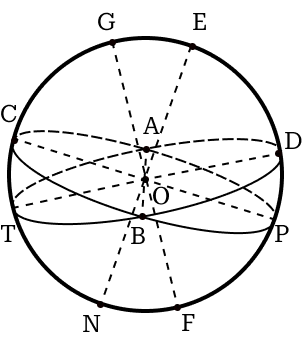
\includegraphics[width=0.2\textwidth]{images/img3} \quad
        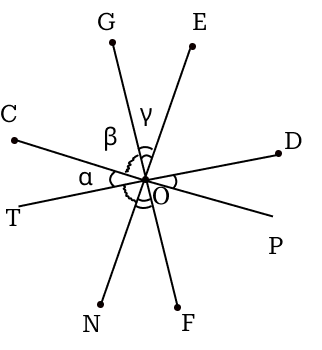
\includegraphics[width=0.2\textwidth]{images/img4}\\
    \end{center}

    1) Так как секущие прямые имеют общую точку, то они пересекаются по прямой $AB$, что следует из аксиом стереометрии.

    2) Восстановим перпендикуляр $OC\bot AB$ в плоскости $(BOC)$ и перпендикуляр $OD \bot AB$ в плоскости $BOD$.
    Проведем прямые, соединяющие полюсы $GF$ и $EN$, так как прямая $AB$ лежит в плоскостях сечений,
    то $CF \bot AB$ и $EN \bot AB$.

    3) $OC \bot AB$, $OD \bot AB$, $GF \bot AB$, $EN \bot AB$,
    тогда эти прямые ($OC, OD, GF, EN$) лежат в плоскости $(COE)$, перпендикулярной прямой $AB$.

    4) Вынесем планиметрический чертеж, на котором $\angle COT = \alpha$ - линейный угол двугранного угла $CABT$,
    который равен углу между секущими плоскостями.
    Так как $GF \bot (TOA)$, то $GF \bot TD \subset (TOA)$ и так как $EN \bot (COP)$, то $EN \bot CP \subset (COP)$.
    Получаем, что $\beta = 90^\circ - \alpha = \angle COT$

    5) Таким образом:
    \[
        2\beta + \alpha + \gamma = 180^{\circ}
    \]
    \[
        180^{\circ} - 2\alpha + \alpha + \gamma = 180 ^{\circ}
    \]
    \[ \alpha = \gamma \]

    Ответ: $\alpha$\\


    \begin{center}
        \textbf{Прямые, полюсы, поляры}
    \end{center}

    \textbf{№3}
    Угол между двумя секущими плоскостями равен $\alpha$.
    Чему равен угол между двумя прямыми,
    каждая из которых соединяет полюсы соответсвующий плоскостей?

    \textbf{Решение}\\

    \begin{center}
        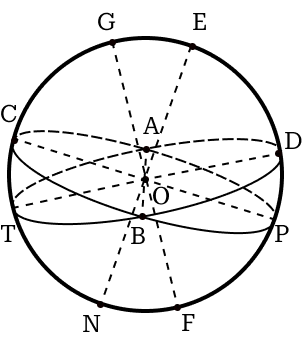
\includegraphics[width=0.2\textwidth]{images/img1} \quad
        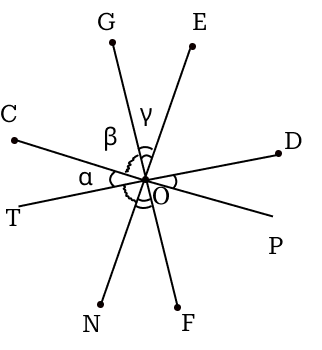
\includegraphics[width=0.2\textwidth]{images/img2}\\
    \end{center}

    1) Так как секущие прямые имеют общую точку, то они пересекаются по прямой $AB$, что следует из аксиом стереометрии.

    2) Восстановим перпендикуляр $OC\bot AB$ в плоскости $(BOC)$ и перпендикуляр $OD \bot AB$ в плоскости $BOD$.
    Проведем прямые, соединяющие полюсы $GF$ и $EN$, так как прямая $AB$ лежит в плоскостях сечений,
    то $CF \bot AB$ и $EN \bot AB$.

    3) $OC \bot AB$, $OD \bot AB$, $GF \bot AB$, $EN \bot AB$,
    тогда эти прямые ($OC, OD, GF, EN$) лежат в плоскости $(COE)$, перпендикулярной прямой $AB$.

    4) Вынесем планиметрический чертеж, на котором $\angle COT = \alpha$ - линейный угол двугранного угла $CABT$,
    который равен углу между секущими плоскостями.
    Так как $GF \bot (TOA)$, то $GF \bot TD \subset (TOA)$ и так как $EN \bot (COP)$, то $EN \bot CP \subset (COP)$.
    Получаем, что $\beta = 90^\circ - \alpha = \angle COT$

    5) Таким образом:
    \[
        2\beta + \alpha + \gamma = 180^{\circ}
    \]
    \[
        180^{\circ} - 2\alpha + \alpha + \gamma = 180 ^{\circ}
    \]
    \[ \alpha = \gamma \]

    Ответ: $\alpha$\\


    \textbf{№4}
    Угол между двумя секущими плоскостями равен $\alpha$.
    Чему равен угол между диаметром, соединяющим одну пару полюсов одной плоскости, и другой плоскостью?

    \textbf{Решение}\\

    Исходя из задач 7 и 9 получаем следующий планиметрический чертёж:

    \begin{center}
        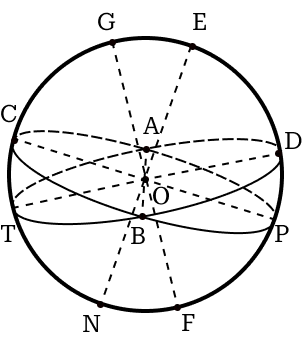
\includegraphics[width=0.2\textwidth]{images/img7} \quad
        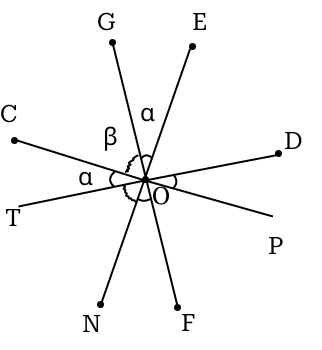
\includegraphics[width=0.2\textwidth]{images/img8}\\
    \end{center}

    1) Необходимо найти угол $\beta$, так как если из $G$ опустить перпендикуляр к $CP$, то он будет перпендикулярен
    плоскости сечения, так как будет перпендикулярен двум пересекающимся прямым $AB$ и $CP$.

    2) $\beta = 90^\circ - \alpha$

    Ответ: $90^\circ - \alpha$\\


    \textbf{№ 5}
    Чему равна площадь евклидового четырехугольника, образованного двумя полисами и диаметрально противоположными точками поляры,
    если радиус сферы $R$.

    \textbf{Решение}\\

    \begin{center}
        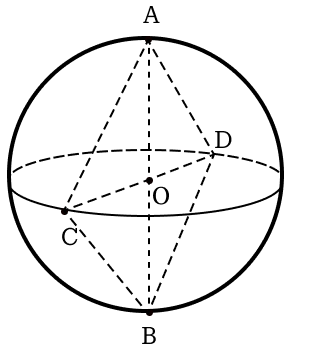
\includegraphics[width=0.2\textwidth]{images/img42}\\
    \end{center}

    1) $CO = DO = AO = BO = R$

    2)
    \[
        S_{ABCD} = S_{\triangle AOC} + S_{\triangle BOC} + S_{\triangle BOD} + S_{\triangle DOA} = 4 S_{\triangle BOC} = 4 * \frac{AO * CO}{2} = 2R^2
    \]

    Ответ: $2R^2$\\


    \begin{center}
        \textbf{Расстояние между точками, углы между прямыми, сферические окружности}
    \end{center}

    \begin{center}
        \textbf{№ 1}
    \end{center}

    На сфере радиуса 7 см построена сферическая окружность радиусом 3 см.
    Чему равен радиус малой окружности, совпадающей с данной?

    \textbf{Решение}\\

    \begin{center}
        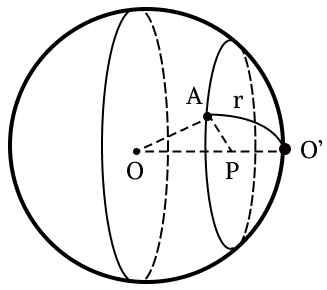
\includegraphics[width=0.2\textwidth]{images/img43}\\
    \end{center}

    1) $OO' = OA = 7$ см, $AP \bot OO'$

    2)
    \[
        r = 7*\angle O'OA \rightarrow \angle O'OA = \frac{3}{7} \text{ см}
    \]

    3)
    \[
        AP = OA * \sin POA = 7 * \sin \frac{3}{7} \text{ см}
    \]

    Ответ: $7\sin \frac{3}{7}$ см

    \begin{center}
        \textbf{№ 2}
    \end{center}

    Проведены две сферические прямые, пересекающиеся под углом $\alpha$,
    перпендикулярно к ним проведена третья сферическая прямая.
    Чему равен угол $\alpha$, если сферическое расстояние между точками пересечения
    двух прямых третьей равно $h$, а радиус сферы равен $R$?

    \textbf{Решение}\\

    \begin{center}
        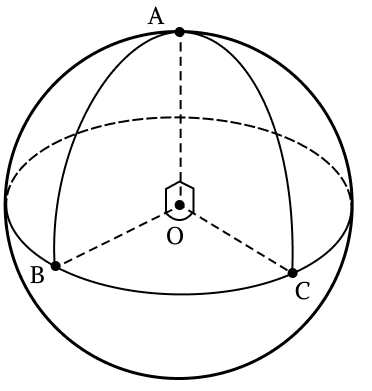
\includegraphics[width=0.2\textwidth]{images/img44}\\
    \end{center}

    \[
        BC = h = \alpha R \rightarrow \alpha = \frac{h}{R}
    \]

    Ответ: $\frac{h}{R}$


    \begin{center}
        \textbf{Фигуры}
    \end{center}

    \begin{center}
        \textbf{№ 8}
    \end{center}
    Две сферические прямые пересекаются под углом $\frac{\pi}{6}$.
    Найдите чему равны площади каждого двуугольника, образованного этими прямыми, и посчитайте их сумму,
    если радиус сферы $R=12$ см.

    \textbf{Решение}\\

    \begin{center}
        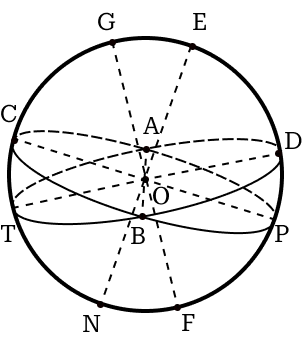
\includegraphics[width=0.2\textwidth]{images/img3}\\
    \end{center}


    1) Пусть $\angle \overline {AB}$ - больший двуугольник, $\overline A, \overline B$ - его углы.
    \[
        \angle A = \frac{\pi}{6}
    \]
    \[ \angle \overline A = \pi - \frac{\pi}{6} = \frac{5\pi}{6}\]

    2)
    \[
        S_{\angle AB} = 2\angle A R ^ 2 = 2 * \frac{\pi}{6} *  144 = 48\pi \text{ см}^2
    \]
    \[
        S_{\angle \overline{AB}} = 2\angle \overline A R ^ 2 = 2 * \frac{5\pi}{6} *  144 = 240\pi \text{ см}^2
    \]

    3)
    \[
        \sum S = 4\pi R ^ 2 = 576 \text{ см}^2
    \]\\

    Ответ: $S_{\angle AB} = 48\pi \text{ см}^2; S_{\angle \overline{AB}} = 240\pi \text{ см}^2; \sum S = 4\pi R ^ 2 = 576 \text{ см}^2$


    \begin{center}
        \textbf{№ 9}
    \end{center}

    Две сферические прямые пересекаются под углом $\alpha$, третья прямая пересекает две проведенные прямые
    под одинаковыми углами.
    Найдите эти углы, если радиус сферы равен $R$, а площадь сферического треугольника, образованного этими прямыми $S$.

    \textbf{Решение}\\

    \begin{center}
        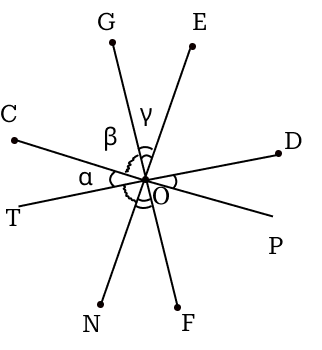
\includegraphics[width=0.2\textwidth]{images/img4}\\
    \end{center}

    1)
    \[
        S_{\triangle ABC} = R^2(\angle A + \angle B + \angle C - \pi) =  R^2(\alpha + 2\angle B - \pi)\rightarrow
        \angle B = \frac{S}{2R^2} - \frac{\alpha- \pi}{2}
    \]

    Ответ: $\frac{S}{2R^2} - \frac{\alpha- \pi}{2} $

    \begin{center}
        \textbf{№ 1}
    \end{center}

     Две сферические прямые пересекаются под углом $\frac{\pi}{2}$.
    Найдите чему равны площади каждого двуугольника, образованного этими прямыми, и посчитайте их сумму,
    если радиус сферы $R=52$ см.

     \textbf{Решение}\\

    \begin{center}
        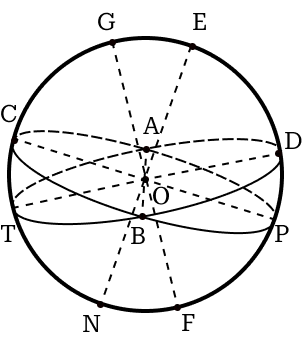
\includegraphics[width=0.2\textwidth]{images/img1}\\
    \end{center}

    1) Образуется четыре равных двуугольника, соответственно их площади равна:
    \[
        S = 2\frac{\pi}{2}R^2 = 2 \frac{\pi}{2} * 52^2 = 2704\pi \text{ см}^2
    \]

    2) Сумма всех двуугольников равна площади сферы, а именно:
    \[
        S_{sph} = 4\pi R^2   =10816 \text{ см}^2
    \]

    Ответ: $2704\pi \text{ см}^2$;  $10816 \text{ см}^2$

    \begin{center}
        \textbf{№ 2}
    \end{center}

    На сфере дан треугольник, два угла которого равны $\frac{\pi}{2}$, а третий равен $\frac{\pi}{3}$.
    Из вершины третьего угла на противолежащую сторону опустили медиану.
    Найдите площади получившихся треугольников, если радиус сферы равен $R$.

    \textbf{Решение}\\

    \begin{center}
        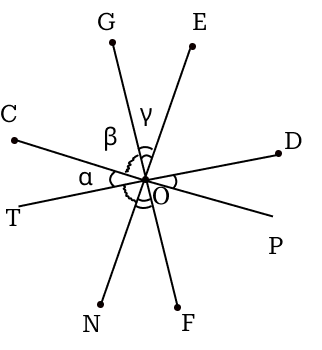
\includegraphics[width=0.2\textwidth]{images/img2}\\
    \end{center}

    1) $AO \bot (BOC)$ по признаку, тогда $(MOA)\bot(BOC)$ по признаку,

    2) \[
           \cup BM = \cup MC \rightarrow \angle BOM = \angle COM = \frac{\pi}{6}
    \]

    3)
    \[
        S = R^2(\angle BOM + \angle AOM + \angle AOB - \pi) = \frac{R^2\pi}{6}
    \]

    Ответ: $\frac{R^2\pi}{6}$

\end{document}
